\documentclass[UTF8]{ctexart}

%\usepackage{indentfirst}           % 首行缩进 
\usepackage[a4paper, left = 3cm, right = 3cm]{geometry}
\usepackage[bf]{titlesec}
\usepackage{listings}               % 代码环境
\usepackage{xcolor}
\lstset{numbers = left,             % 设置行号位置
        numberstyle = \tiny,        % 设置行号大小
        keywordstyle = \color{blue!70},                         % 设置关键字颜色
        commentstyle = \color{red!50!green!50!blue!50},         % 设置注释颜色
        frame = single,             % 设置边框格式
        rulesepcolor = \color{red!20!green!20!blue!20},
        escapeinside = ',          % 逃逸字符,用于显示中文
        xleftmargin = 1em, xrightmargin = 1em, aboveskip = 1em, % 设置边框边距        
        tabsize = 4,                % 设置tab空格数
        showspaces = false,         % 不显示空格
        extendedchars = false,
        flexiblecolumns,            % 字列非等宽
        breaklines                  % 自动将长代码换行排版
        }

\usepackage[colorlinks, linkcolor = black, anchorcolor = black, citecolor = black]{hyperref}            % 目录超链接
\renewcommand{\contentsname}{\centerline{目录}}
\usepackage[nottoc]{tocbibind}      % 章节编号等加入目录
\usepackage{ctex}
\usepackage{graphicx}               % 插图    
\usepackage{subfigure}              % 实现图片并排
\usepackage{float}                  % 强制图片位置
\usepackage{amsmath}                % 数学公式  
\usepackage{fancyvrb}

\usepackage{fancyhdr}                   % 设置页眉页脚
\pagestyle{fancy}
\lhead{编码引论第二次仿真实验报告}
\chead{}
\rhead{无35 \quad 陈馨瑶 \quad 2013011166}
\lfoot{}
\cfoot{\thepage}
\rfoot{}

\title{\vspace*{6cm}编码引论第二次仿真实验报告}
\author{无35 \quad 陈馨瑶 \quad 2013011166}
\date{\today}

\begin{document}

\begin{titlepage}
\maketitle

\thispagestyle{empty}
\end{titlepage}

\setlength{\headheight}{13pt}

\tableofcontents

\newpage

\section{接口及分工}

本次实验所采取的加解密方式为DES,我们小组将实验内容分为如下三个部分,每个部分由一个人完成,由我完成的是第二部分。各部分接口说明如下(这里只列出了本次实验新加入的接口):

\subsection{PART I}

\subsubsection{子密钥生成 keygen}
\begin{itemize}
        \item 输入:key: 64bits original key
        \item 输出:subkeys: 16 cells, each contains one 48bits subkey
\end{itemize}

\subsection{PART II}

\subsubsection{密码函数 Feistel}

\begin{itemize}
        \item 输入:R: Half Block(长度32,logical array),key: 密钥(长度48,logical array)
        \item 输出:feistel\_out: f(R, k)(长度32,logical array)
\end{itemize}

\subsection{PART III}

\subsubsection{加密 encrypt}

\begin{itemize}
        \item 输入:data: 输入数据流,key: 64 位密钥
        \item 输出:encrypted: 加密数据流
\end{itemize}

\subsubsection{解密 decrypt}

\begin{itemize}
        \item 输入:encrypted: 加密数据流,key: 64 位密钥
        \item 输出:data: 解密后数据流
\end{itemize}

\subsubsection{密钥生成 create\_key}

\begin{itemize}
        \item 输入:num: 所需密钥数目,默认为 1,
        \item 输出:key: num 个密钥,每列为一个 64 位密钥
\end{itemize}

\subsubsection{主程序 main}

\begin{itemize}
        \item 计算误比特率。
        \item 以 64 bit 为单位,画出误码图案。
\end{itemize}


\section{模块设计 Feistel}

实验中由我完成的Feistel模块流程如下图所示:
\begin{figure}[H]
    \centering
    \includegraphics[scale = 0.6]{01.png}
\end{figure}   

在DES算法中,Feistel函数的一个输入为以64bit长度分组后的数据的一半,在加密过程中为每一轮的$R_i$,另一输入为当前轮48bit子密钥。Feistel函数的步骤如下:

\begin{itemize}
    \item 扩展置换
    \item 密钥混合
    \item 压缩置换
    \item 重排输出
\end{itemize}

\subsection{扩展置换 Expansion}
将输入的32bit数据扩展成48bit。采用的方式为:首先将该32bit数据分成8组,每组4bit,然后在这4bit头尾加上上一组和下一组与之紧邻的1bit数据,将得到的每组6bit数据拼接成48bit,由此完成扩展。

这一步可以采用的完成方式有查找表和循环,我采用的是循环方式。需要注意的是最后一组的末尾加上的是第一位,第一组的头部加上的是最后一位。

\subsection{密钥混合 Key-mixing}
这一步直接将上一步得到的48bit数据和当前轮子密钥进行逐位异或即可。

\subsection{压缩置换 Substitution}
将异或得到的48bit数据分成8个6bit块,利用每个块的6bit数据运算得到4bit输出。

这里的运算方式为查找表。实验时,利用randi生成8个元素范围在0-15的矩阵,每个块对应一个不同的$4 \times 16$矩阵,

\subsection{重排输出 Permutation}
利用查找表方式,将上一步得到的每块4bit打散到4个不同的块中,最后得到32bit数据作为输出。

\section{仿真结果}

\subsection{误比特率}
误比特率曲线如下图所示,其中,蓝色表示加密过的结果,红色表示未经过加密的结果。

\begin{figure}[H]
    \centering
    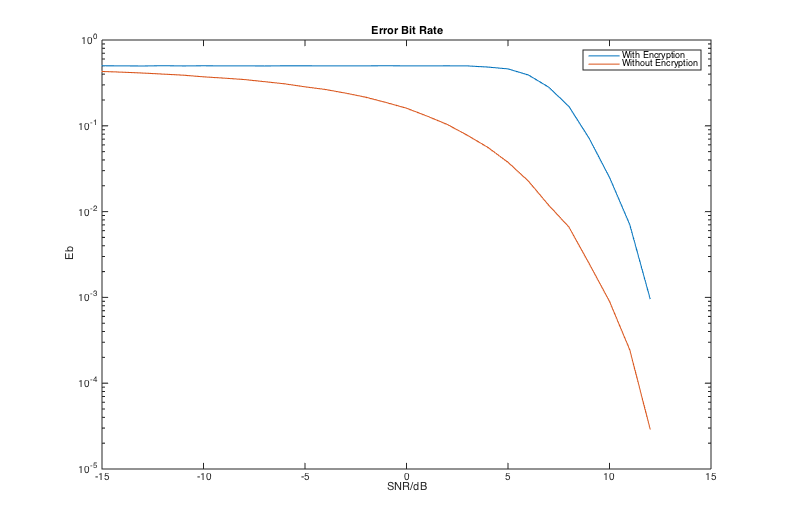
\includegraphics[width = 0.8\textwidth]{error_bit_rate.png}
\end{figure}

从图中可以看到,蓝色曲线和红色曲线的变化趋势一致,但在相同SNR下经过加密的信号的误比特率明显高于未经加密的信号,这说明在经过加密后,由于信道噪声带来的误码得到了放大。基于窃听者的信道质量较接收方差得多的假设,此次实验中所设计的加密机制的确起到了保障信息安全的作用。

\subsection{误码图案}
为了更直观地说明加密的效果,我们画出了SNR = 1dB时经过加密和未经加密的误码图案,如下:

\begin{figure}[H]
    \centering
    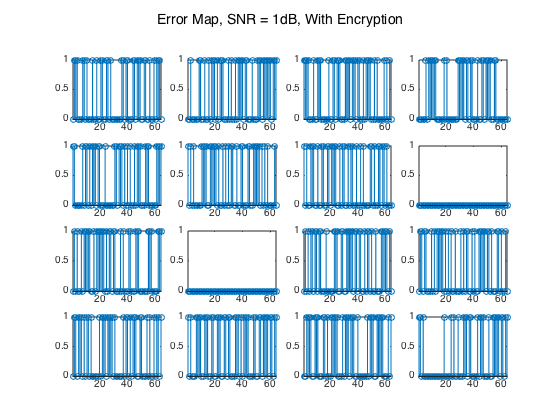
\includegraphics[width = 0.8\textwidth]{error_map_1dB_with.png}
    \caption{SNR=1dB,经过加密}
\end{figure}

\begin{figure}[H]
    \centering
    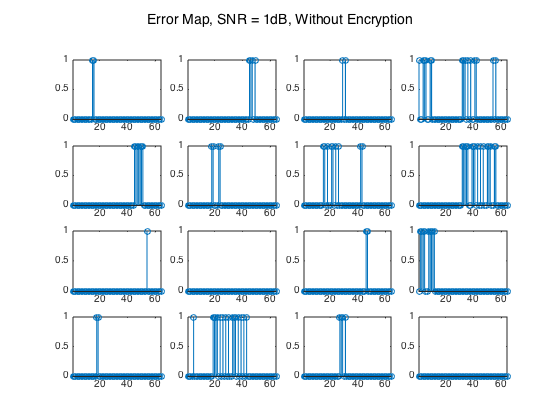
\includegraphics[width = 0.8\textwidth]{error_map_1dB_without.png}
    \caption{SNR=1dB,未经加密}
\end{figure}

两图对比可以看出,其实当SNR = 1dB时由信道噪声本身造成的误码已经很少,而且在大多数情况下都是属于零散的突发错,然而,在经过加密后,误码几乎完全是以“误块”形式出现的。这说明在解密时,很小的一点(几比特)偏差就会影响与其相邻的很多比特数据。这也说明了设计的加密机制的雪崩效应足够好。


\section{附:代码}
我所完成部分的代码如下:Feistel.m
\lstinputlisting[language = Matlab]{Feistel.m}


\end{document}